% Copyright 2021 Joel Feldman, Andrew Rechnitzer and Elyse Yeager, except where noted.
% This work is licensed under a Creative Commons Attribution-NonCommercial-ShareAlike 4.0 International License.
% https://creativecommons.org/licenses/by-nc-sa/4.0/

\section*{2.13: Mean Value Theorem}

\begin{frame}{Table of Contents}
\mapofcontentsB{\bn}
\end{frame}

%----------------------------------------------------------------------------------------
%----------------------------------------------------------------------------------------
%----------------------------------------------------------------------------------------
%----------------------------------------------------------------------------------------
\begin{frame}[t]{Rolle's Theorem}
\note{Draw several functions passing through these two points. Start with continuous, differentiable, and point out there is always a flat spot. Ask students: \textit{must} there always be a flat spot? Give examples with corners, discontinuities.}
\begin{center}
\begin{tikzpicture}
\myaxis{x}{1}{4}{y}{2}{3}
\draw (1,1) node[vertex]{};
\draw (3,1) node[vertex]{};
\end{tikzpicture}
\end{center}
\end{frame}
%----------------------------------------------------------------------------------------
%----------------------------------------------------------------------------------------
\begin{frame}[t]
\begin{block}{Rolle's Theorem -- Theorem~\eref{text}{thm:DIFFrolle}}
Let $a$ and $b$ be real numbers, with $a<b$. And
let $f$ be a function with the properties:
\begin{itemize}
\item[\textbullet]~ \onslide<2->{$f(x)$ is continuous for every $x$ with $a \leq x \leq b$;}
\item[\textbullet]~ \onslide<3->{$f(x)$ is differentiable when $a<x<b$;}
\item[\textbullet]~ and $f(a)=f(b)$.
\end{itemize}
Then there exists a number $c$ with $a<c<b$ such that 
\[f'(c)=0.\] 
\end{block}
\end{frame}
%----------------------------------------------------------------------------------------
\begin{frame}[t]
\begin{block}{Rolle's Theorem -- Theorem~\eref{text}{thm:DIFFrolle}}
Let $f(x)$ be \textcolor{M3}{continuous} on the interval $[a,b]$, \textcolor{M3}{differentiable} on $(a,b)$,  \textcolor{M3}{and let $f(a)=f(b)$.} Then there is a number $c$ strictly between $a$ and $b$ such that
$f'(c)=\textcolor{M3}{0}$.
\end{block}
\vfill

Example: Let $f(x)=x^3-2x^2+1$, and observe $f(2)=f(0)=1$. Since $f(x)$ is a polynomial, it is continuous and differentiable everywhere.

\begin{multicols}{2}
\begin{tikzpicture}
\myaxis{x}{0}{3}{y}{0}{2}
\draw (0,1) node[vertex]{};
\draw (2,1) node[vertex]{};
\draw (2,.2)--(2,-.2) node[below]{$2$};
\onslide<2-|handout:0>{\draw[thick, C1] plot[domain=0:2, samples=50](\x,{\x*\x*\x-2*\x*\x+1});}
\end{tikzpicture}
\columnbreak\color{answercolor}

\onslide<2|handout:0>{\begin{align*}
0=f'(x)&=3x^2-4x\\
&=x(3x-4)\\
x&=0 \mbox{ and } \boxed{x=\frac43}\\
f'\left(\frac43\right)&=0
\end{align*}}
\end{multicols}


\note<1>{By Rolle's Theorem, we are guaranteed that $f'(x)=0$ for \textit{some} $x$ in the interval $(0,2)$. Which $x$ fulfils this guarantee?}
\end{frame}
%----------------------------------------------------------------------------------------
\begin{frame}
\begin{block}{Rolle's Theorem -- Theorem~\eref{text}{thm:DIFFrolle}}
Let $f(x)$ be \textcolor{M3}{continuous} on the interval $[a,b]$, \textcolor{M3}{differentiable} on $(a,b)$,  \textcolor{M3}{and let $f(a)=f(b)$.} Then there is a number $c$ strictly between $a$ and $b$ such that
$f'(c)=\textcolor{M3}{0}$.
\end{block}
\vfill
\only<1-4>{\QuestionBar{1}{2}\AnswerYes}
\only<5>{\AnswerBar{1}{2}}
\only<6-7>{\QuestionBar{2}{2}\AnswerYes}
\only<8-9>{\AnswerBar{2}{2}}
\note<4>{If there's not much agreement, flash the two examples, then let students vote again.}
\begin{multicols}{2}
\begin{tikzpicture}
\myaxis{x}{0}{4}{y}{0}{2}
\draw (1,1) node[vertex]{};
\draw (3,1) node[vertex]{};
\draw (1,.2)--(1,-.2) node[below]{$a$};
\draw (3,.2)--(3,-.2) node[below]{$b$};
\onslide<2|handout:0>{\draw[thick, C1] plot[domain=1:3] (\x,{sin(pi*(\x-1)/2 r)+1});
\draw[M4] (2,2) node[vertex]{};
\draw[M4] (1.5,2)--(2.5,2);}
\onslide<3|handout:0>{\draw[thick, C1] plot[domain=1:3] (\x,{.75*sin(pi*(\x-1) r)+1});
\draw[M4, opacity=0.75] (1.5,1.75) node[vertex]{};
\draw[M4] (1,1.75)--(2,1.75);
\draw[M4, opacity=0.75] (2.5,.25) node[vertex]{};
\draw[M4] (2,.25)--(3,.25);
}
\onslide<7|handout:0>{\draw[C1, ultra thick] (1,1)--(3,1);}
\end{tikzpicture}

Suppose $a<b$ and \textcolor{M3}{$f(a)=f(b)$}, $f(x)$ is \textcolor{M3}{continuous} over $[a,b]$, and $f(x)$ is \textcolor{M3}{differentiable} over $(a,b)$.\columnbreak

\only<1-5>{How many different values of $x$ between $a$ and $b$ have $f'(x)=0$?\vfill
\begin{enumerate}[A.]
\item 0 or 1
\item 1
\item 0, 1, or more 
\alert<5-|handout:0>{\item 1 or more }
\item I'm not sure
\end{enumerate}}
\only<6-|handout:0>{Can $f$ have an \textcolor{M4}{infinite number} of points where $f'(x)=0$ between $a$ and $b$?\vfill
\begin{itemize}
\alert<9-|handout:0>{\item[A.] Sure! 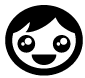
\includegraphics[height=6mm]{Clipart/agree}}
\item[B.] No way! 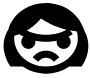
\includegraphics[height=6mm]{Clipart/disagree}
\item[C.] Only if $a$ and $b$ are infinitely far apart  
\includegraphics[height=6mm]{Clipart/nope}
\item[D.] I'm not sure 
\end{itemize}
\index{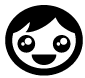
\includegraphics[height=5mm]{Clipart/agree}
\href{https://thenounproject.com/term/love-it/2073299/}{`love it'} by
\href{https://thenounproject.com/JS.Beaulieu/}{JS Beaulieu} is licensed under
 \CCBYthree~ (accessed 6 July 2021)}
 
\index{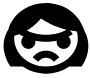
\includegraphics[height=5mm]{Clipart/disagree}
\href{https://thenounproject.com/term/strongly-disagree/2073304/}{`strongly disagree'}
by
\href{https://thenounproject.com/JS.Beaulieu/}{JS Beaulieu} is licensed under
\CCBYthree~ (accessed 6 July 2021)}

\index{
\includegraphics[height=5mm]{Clipart/nope} 
\href{https://thenounproject.com/term/nope/1766945/}{`nope'}
by
\href{https://thenounproject.com/allielamb/}{Allie} is licensed under
\CCBYthree~  (accessed 6 July 2021)}
}
\note<8>{If most students choose the wrong answer, show them the example, vote again. They'll likely ask whether this is the \textit{only} example. We've seen infinite wiggling before.}
\end{multicols}
\end{frame}
%----------------------------------------------------------------------------------------
%----------------------------------------------------------------------------------------
\begin{frame}[t]\AnswerSpace
\begin{block}{Rolle's Theorem -- Theorem~\eref{text}{thm:DIFFrolle}}
Let $f(x)$ be \textcolor{M3}{continuous} on the interval $[a,b]$, \textcolor{M3}{differentiable} on $(a,b)$,  \textcolor{M3}{and let $f(a)=f(b)$.} Then there is a number $c$ strictly between $a$ and $b$ such that
$f'(c)=\textcolor{M3}{0}$.
\end{block}

\begin{QuestionSet}
\SetQuestion{\AnswerYes
\begin{multicols}{2}
Suppose $f(x)$ is continuous and differentiable for all real numbers, and $f(x)$ has precisely seven roots, all different. How many roots does $f'(x)$ have?\columnbreak

\begin{itemize}
\item[A.] precisely six
\item[B.] precisely seven
\item[C.] at most seven
\item[D.] at least six
\end{itemize}
\end{multicols}
}
\SetAnswer{
\begin{multicols}{2}
Suppose $f(x)$ is continuous and differentiable for all real numbers, and $f(x)$ has precisely seven roots, all different. How many roots does $f'(x)$ have?\columnbreak

\begin{itemize}
\item[A.] precisely six
\item[B.] precisely seven
\item[C.] at most seven
\alert{\item[D.] at least six}
\end{itemize}
\end{multicols}
}
%
\SetQuestion{\AnswerYes\begin{multicols}{2}
Suppose $f(x)$ is continuous and differentiable for all real numbers, and $f'(x)$ is also continuous and differentiable for all real numbers, and $f(x)$ has precisely seven roots, all different. How many roots does $f''(x)$ have?
\columnbreak
\begin{itemize}
\item[A.] precisely six
\item[B.] precisely five
\item[C.] at most five
\item[D.] at least five
\end{itemize}
\end{multicols}
}
\SetAnswer{\begin{multicols}{2}
Suppose $f(x)$ is continuous and differentiable for all real numbers, and $f'(x)$ is also continuous and differentiable for all real numbers, and $f(x)$ has precisely seven roots, all different. How many roots does $f''(x)$ have?
\columnbreak
\begin{itemize}
\item[A.] precisely six
\item[B.] precisely five
\item[C.] at most five
\alert{\item[D.] at least five}
\end{itemize}
\end{multicols}}
%
\SetQuestion{\AnswerYes
\begin{multicols}{2}
Suppose $f(x)$ is continuous and differentiable for all real numbers, and there are precisely three places where $f'(x)=0$. How many distinct roots does $f(x)$ have?\columnbreak
\begin{itemize}
\item[A.] at most three
\item[B.] at most four
\item[C.] at least three
\item[D.] at least four
\end{itemize}
\end{multicols}
}
\SetAnswer{
\begin{multicols}{2}
Suppose $f(x)$ is continuous and differentiable for all real numbers, and there are precisely three places where $f'(x)=0$. How many roots does $f(x)$ have?\columnbreak
\begin{itemize}
\item[A.] at most three
\alert{\item[B.] at most four}
\item[C.] at least three
\item[D.] at least four
\end{itemize}
\end{multicols}
}
%
\SetQuestion{\AnswerYes
\begin{multicols}{2}
Suppose $f(x)$ is continuous and differentiable for all real numbers, and $f'(x)=0$ for precisely three values of $x$. How many distinct values $x$ exist with $f(x)=17$?\columnbreak
\begin{itemize}
\item[A.] at most three
\item[B.] at most four
\item[C.] at least three
\item[D.] at least four
\end{itemize}
\end{multicols}
}
\SetAnswer{
\begin{multicols}{2}
Suppose $f(x)$ is continuous and differentiable for all real numbers, and $f'(x)=0$ for precisely three values of $x$. How many distinct values $x$ exist with $f(x)=17$?\columnbreak
\begin{itemize}
\item[A.] at most three
\alert{\item[B.] at most four}
\item[C.] at least three
\item[D.] at least four
\end{itemize}
\end{multicols}
}
\end{QuestionSet}
\end{frame}
%----------------------------------------------------------------------------------------

%----------------------------------------------------------------------------------------
\begin{frame}[t]{Applications of Rolle's Theorem}
\only<1>{\QuestionBar{1}{3}\AnswerYes}
\only<2-4>{\AnswerBar{1}{3}}

Prove that the function $f(x)=x^3+x-1$ has at most one real root.\\[1em]\pause
\answer{
\only<2>{
\begin{center}\begin{tikzpicture}
\color{C1}
\draw (0,3) node(r){\parbox{4cm}{\raggedright How many roots does $f(x)$ have?}};
\draw (-3,0) node[below](a){\parbox{3cm}{\raggedright  $f'(c)=0$ somewhere}};
\draw (3,0) node[below](b){\parbox{3cm}{\raggedright anything can happen}};
\draw[thick, ->,M3] (r)--(a) node[midway, left, inner sep=1mm, fill=white,draw]{2 or more};
\draw[thick, ->,M3] (r)--(b) node[midway, right, inner sep=1mm, fill=white,draw]{0 or 1};
\end{tikzpicture}\end{center}}

\color{answercolor}


\only<3>{
Note that $f(x)$ is \textcolor{C3}{continuous}  and \textcolor{C3}{differentiable} over all real numbers. So, by Rolle's Theorem, if it has two roots, then $f'(x)=0$ for some $x$.\vfill

$f'(x)=3x^2+1$, and this is always at least one, so it's never zero. Therefore, by Rolle's Theorem, $f(x)$ does not have two roots; so it has at most one.

\[0 \qquad 1 \qquad \xcancel2 \qquad \xcancel3 \qquad \xcancel4 \qquad \xcancel5 \qquad \cdots\]
\note<3>{It's often not obvious to students that the opposite of ``at least two" is ``at most one," hence the list of cancelled numbers.}
}
\only<4>{
Logical Structure:
\begin{multicols}{2}
\textbullet~ If $A$ is true, then $B$ is true.\\
\textbullet~ $B$ is false.\\
\textbullet~ Therefore, $A$ is false.\\
\pause\columnbreak
\textbullet~ If $f(x)$ has two (or more) roots, then $f'(x)$ has a root.\\
\textbullet~ $f'(x)$ does not have a root.\\
\textbullet~ Therefore, $f(x)$ does not have two (or more) roots.\\
\end{multicols}}
}%answer

\only<5->{\color{C1}How would you show that $f(x)$ has \emph{precisely} one real root?\\[1em]}
\only<5>{\QuestionBar{2}{3}\AnswerYes}
\answer{
\only<6->{\AnswerBar{2}{3} \color{answercolor}}
\only<6>{
We know it has 0 or 1 root. 
\[\boxed{0 \qquad 1} \qquad \xcancel2 \qquad \xcancel3 \qquad \xcancel4 \qquad \xcancel5 \qquad \cdots\]
We need to show it has ``not zero" roots. So, we would find a root.}

\only<7->{Inconveniently, it's hard to actually solve $0=x^3+x-1$. So, we use the IVT (Section \eref{text}{sec_1_6}).

\begin{block}{Intermediate Value Theorem (IVT) -- Theorem~\eref{text}{thm ivt}}
Let $a<b$ and let $f(x)$ be continuous over $[a,b]$. If $y$ is any number between $f(a)$ and $f(b)$, then there exists $c$ in $(a,b)$ such that $f(c)=y$. 
\end{block}}

\only<8>{Since $f(1)>0$ and $f(0)<0$, and $f(x)$ is a continuous function, by the IVT $f(x)$ has a root (between 0 and 1).

\begin{center}\begin{tikzpicture}
\myaxis{x}{4}{4}{}{.75}{.5}
\xcoord{3}{1}
\draw(3,.5)node[vertex]{};
\draw(0,-.5)node[vertex]{};
\end{tikzpicture}\end{center}}
}%answer

\unote{Example~\eref{text}{eg_2_13_2}}
\end{frame}

%------------------------------------------------------------------%----------------------------------------------------------------------------------------
%----------------------------------------------------------------------------------------
\begin{frame}[t]
\only<1>{\QuestionBar{3}{3}\AnswerYes}
\only<2->{\AnswerBar{3}{3}}
Use Rolle's Theorem to show that the function $f(x)=\frac{1}{3}x^3+3x^2+9x-3$ has at most two distinct real roots.\\[1em]\color{answercolor}

\only<2|handout:0>{Again we use the structure:
\begin{itemize}\color{answercolor}
\item If $f(x)$ has three distinct roots, then $f'(x)$ has two (or more) distinct roots. 
\begin{tikzpicture}
\myaxis{}{2}{2}{}{.25}{.5}
\foreach \x in {-1.5,-.5,1.5}\draw (\x,0) node[C1,vertex]{};
\draw (-1.5,0) to[bend left] (-.5,0);
\draw (-.5,0) to[bend right] (1.5,0);
\end{tikzpicture}
\item $f'(x)$ does not have two (or more) distinct roots.
\item Therefore, $f(x)$ does not have three distinct roots.
\end{itemize}\vfill

So, all we need to do is make sure the conditions of Rolle's Theorem are satisfied, and show that $f'(x)$ does not have two (or more) distinct roots.}

\only<3|handout:0>{Since $f(x)$ is continuous and differentiable over all real numbers, the conditions of Rolle's Theorem are satisfied.\vfill

$f'(x)=x^2+6x+9=(x+3)^2$, which only has ONE root, namely $x=-3$.\vfill

Therefore, $f'(x)$ does not have two distinct roots, so $f(x)$ does not have 
three distinct roots.\vfill

So, $f(x)$ has at most two distinct roots.}
\end{frame}
%----------------------------------------------------------------------------------------
%----------------------------------------------------------------------------------------

%----------------------------------------------------------------------------------------
%----------------------------------------------------------------------------------------
\begin{frame}[t]{Average Rate of Change}
\only<1>{\AnswerYes}
\begin{multicols}{2}

\begin{tikzpicture}
\myaxis{x}{0}{4}{y}{0}{2}
\draw (1,1) node[vertex]{};
\draw (3,1) node[vertex]{};
\draw (1,.2)--(1,-.2) node[below]{$1$};
\draw (3,.2)--(3,-.2) node[below]{$3$};
\draw (.2,1.75)--(-.2,1.75) node[left]{$5$};
\draw (.2,1)--(-.2,1) node[left]{$3$};
\draw (.2,.25)--(-.2,.25) node[left]{$1$};
\draw[thick, C1] plot[domain=1:3] (\x,{.75*sin(pi*(\x-1) r)+1});

\onslide<3-|handout:0>{\draw[M4, opacity=0.75] (1.5,1.75) node[vertex]{};
\draw[M4, dashed] (1,1.75)--(2,1.75);
\draw[M4, dashed] (1,1)--(3,1);
}
\end{tikzpicture}
\vfill
\only<2-|handout:0>{ \textcolor{answercolor}{\[\frac{\Delta y}{\Delta x} = \frac{3-3}{3-1}=\frac{0}{2}=0\]}}
\vfill
\columnbreak

What is the \textcolor{M4}{average rate of change} of $f(x)$ from $x=1$ to $x=3$?\\[1em]
\begin{itemize}
\alert<2-|handout:0>{\item[A.] 0 }
\item[B.] 1
\item[C.] 2 
\item[D.] 4
\item[E.] I'm not sure
\end{itemize}
\end{multicols}
\note<3>{Rolle's Theorem tells us there is a spot where the derivative is 0; in this case, that's the same as the average rate of change.}
\end{frame}
%----------------------------------------------------------------------------------------
%----------------------------------------------------------------------------------------
\begin{frame}[t]{Average Rate of Change}
\note<1>{Want a visual example that's simpler than the last one in order to illustrate Average RoC theorem. This also gives students a second chance to get the average RoC correct.}
\only<1>{\AnswerYes}
\begin{multicols}{2}
\begin{tikzpicture}
\myaxis{x}{0}{4}{y}{0}{2}
\draw (1,1) node[vertex]{};
\draw (3,1) node[vertex]{};
\draw (1,.2)--(1,-.2) node[below]{$2$};
\draw (3,.2)--(3,-.2) node[below]{$7$};
\draw (.2,2)--(-.2,2) node[left]{$30$};
\draw (.2,1)--(-.2,1) node[left]{$15$};
\draw[thick, C1] plot[domain=1:3] (\x,{sin(pi*(\x-1)/2 r)+1});

\onslide<3-|handout:0>{\draw[M4,  opacity=0.75] (2,2) node[vertex]{};
\draw[M4, dashed] (1.5,2)--(2.5,2);
\draw[M4, dashed] (1,1)--(3,1);}
\end{tikzpicture}
\vfill
\onslide<2-|handout:0>{\[\textcolor{answercolor}{\frac{\Delta y}{\Delta x} = \frac{15-15}{7-2}=\frac{0}{5}=0}\]}
\vfill
\columnbreak

What is the \textcolor{M4}{average rate of change} of $f(x)$ from $x=2$ to $x=7$?\\[1em]
\begin{itemize}
\alert<2-|handout:0>{\item[A.] 0 }
\item[B.] 3
\item[C.] 5 
\item[D.] 15
\item[E.] I'm not sure
\end{itemize}
\end{multicols}
\end{frame}
%----------------------------------------------------------------------------------------
%----------------------------------------------------------------------------------------
\begin{frame}[t]
\begin{block}{Rolle's Theorem and Average Rate of Change}
Suppose $f(x)$ is \textcolor{M3}{continuous} on the interval $[a,b]$, \textcolor{M3}{differentiable} on the interval $(a,b)$, and \textcolor{M3}{$f(a)=f(b)$}. Then there exists a number $c$ strictly between $a$ and $b$ such that
\[f'(c)=0=\textcolor{M4}{\frac{f(b)-f(a)}{b-a}}.\]
\end{block}
So there exists a point where the derivative is the same as the average rate of change.
\end{frame}
%----------------------------------------------------------------------------------------
%----------------------------------------------------------------------------------------
\begin{frame}[t]
\mode<beamer>{\begin{center}
\only<1-2>{
\begin{tikzpicture}
\only<1>{\myaxis{x}{0}{4}{y}{0}{2}}
\draw (1,1) node[vertex]{};
\draw (3,1) node[vertex]{};
\draw[thick, C1] plot[domain=1:3] (\x,{sin(pi*(\x-1)/2 r)+1});
{\draw[M4,  opacity=0.75] (2,2) node[vertex]{};
\draw[M4, dashed] (1.5,2)--(2.5,2);
\draw[M4, dashed] (1,1)--(3,1);}
\end{tikzpicture}}
\only<3>{
\begin{tikzpicture}[rotate=-30]
\draw (1,1) node[vertex]{};
\draw (3,1) node[vertex]{};
\draw[thick, C1] plot[domain=1:3] (\x,{sin(pi*(\x-1)/2 r)+1});
{\draw[M4,  opacity=0.75] (2,2) node[vertex]{};
\draw[M4, dashed] (1.5,2)--(2.5,2);
\draw[M4, dashed] (1,1)--(3,1);}
\end{tikzpicture}
}
\end{center}}
\end{frame}
%----------------------------------------------------------------------------------------
\begin{frame}
\begin{block}{Mean Value Theorem -- Theorem~\eref{text}{thm:DIFFmvt}}

Let $f(x)$ be \textcolor{M3}{continuous} on the interval $[a,b]$ and \textcolor{M3}{differentiable} on $(a,b)$. Then there is a number $c$ strictly between $a$ and $b$ such that:
\[\begin{tikzpicture}[rotate=-30]
\draw (1,1) node[vertex]{};
\draw (3,1) node[vertex]{};
\draw[thick, C1] plot[domain=1:3] (\x,{sin(pi*(\x-1)/2 r)+1});
{\draw[M4,  opacity=0.75] (2,2) node[vertex]{};
\draw[M4, dashed] (1.5,2)--(2.5,2);
\draw[M4, dashed] (1,1)--(3,1);}
\end{tikzpicture}\hspace{1cm} f'(c)=\textcolor{M4}{\frac{f(b)-f(a)}{b-a}}\]
That is: there is some point $c$ in $(a,b)$ where the instantaneous rate of change of the function is equal to the average rate of change of the function on the interval $[a,b]$.
\end{block}

\end{frame}
%----------------------------------------------------------------------------------------
\begin{frame}[t]
\begin{QuestionSet}
\SetQuestion{\AnswerYes
Suppose you are driving along a long, straight highway with no shortcuts. The speed limit is 100 kph. A police officer notices your car going 90 kph, and uploads your plate and the time they saw you to their database. 150 km down this same straight road, 75 minutes later, another police officer notices your car going 85kph, and uploads your plates to the database. Then they pull you over, and give you a speeding ticket. Why were they justified?


\includegraphics[height=1cm]{Clipart/speedometer}
\index{
\includegraphics[height=5mm]{Clipart/speedometer}
\href{https://thenounproject.com/term/speedometer/4040085/}{`Speedometer'}
by
\href{https://thenounproject.com/pockerironsv/}{Serhii Smirnov}
is licensed under
 \CCBYthree~  (accessed 6 July 2021)}

\vfill
}
\SetAnswer{\color{answercolor}
You travelled $150$ km in 75 minutes. Since a moving car has a position that is continuous and differentiable, the MVT tells us that at some point, your instantaneous velocity was $\frac{150}{75}$ kilometers per minute, which works out to $\frac{150\cdot 60}{75 }=120$ kph. So even though you weren't speeding when the officers saw you, you were definitely speeding some time in between.
\vfill
Alternately, if you were going at most 100kph, then you would need
at least 90 minutes to travel 150 kilometers.
\vfill}
%
\SetQuestion{\AnswerYes
According to \href{https://blog.americanexpedition.us/canada-geese-infographic/}
{\textcolor{C1}{this website}}, Canada geese may fly 1500 miles in a single day under favorable conditions. It also says their top speed is around 70mph. Does this seem like a typo? (If it contradicts the Mean Value Theorem, it's probably a typo.)


\includegraphics[height=1.5cm]{Clipart/goose}
\index{ 
\includegraphics[height=5mm]{Clipart/goose}
\href{https://thenounproject.com/term/goose/1175331/}{`Goose'}
by
\href{https://thenounproject.com/idsmaryb/}{Mary B}
is licensed under
 \CCBYthree~ 
(accessed 6 July 2021)}

\vfill
}
\SetAnswer{\color{answercolor}
We can assume that the position of a goose is continuous and differentiable. Then the MVT tells us that a goose that travels $1500$ miles in a day (24 hours) achieves, at some instant, a speed of $\frac{1500}{24}$ mph. Since $\frac{1500}{24}=62.5$, these two facts seem compatible (and amazing!).
}
%
\SetQuestion{\AnswerYes
The record for fastest wheel-driven land speed is around 700 kph. 
\footnote
{(at time of writing) George Poteet, \url{https://en.wikipedia.org/wiki/Wheel-driven_land_speed_record}}
 However, non-wheel driven cars (such as those powered by jet engines) have achieved higher speeds.
 \footnote{\url{https://en.wikipedia.org/wiki/Land_speed_record}}

Suppose a driver of a jet-powered car starts a 10km race at 12:00, and finishes at 12:01.
Did they beat 700kph?

}
\SetAnswer{\color{answercolor}
Maybe, but not necessarily. We are only guaranteed by the MVT that at some point they reached the following speed: $\frac{10}{(1/60)}=600$ kph.
\vfill
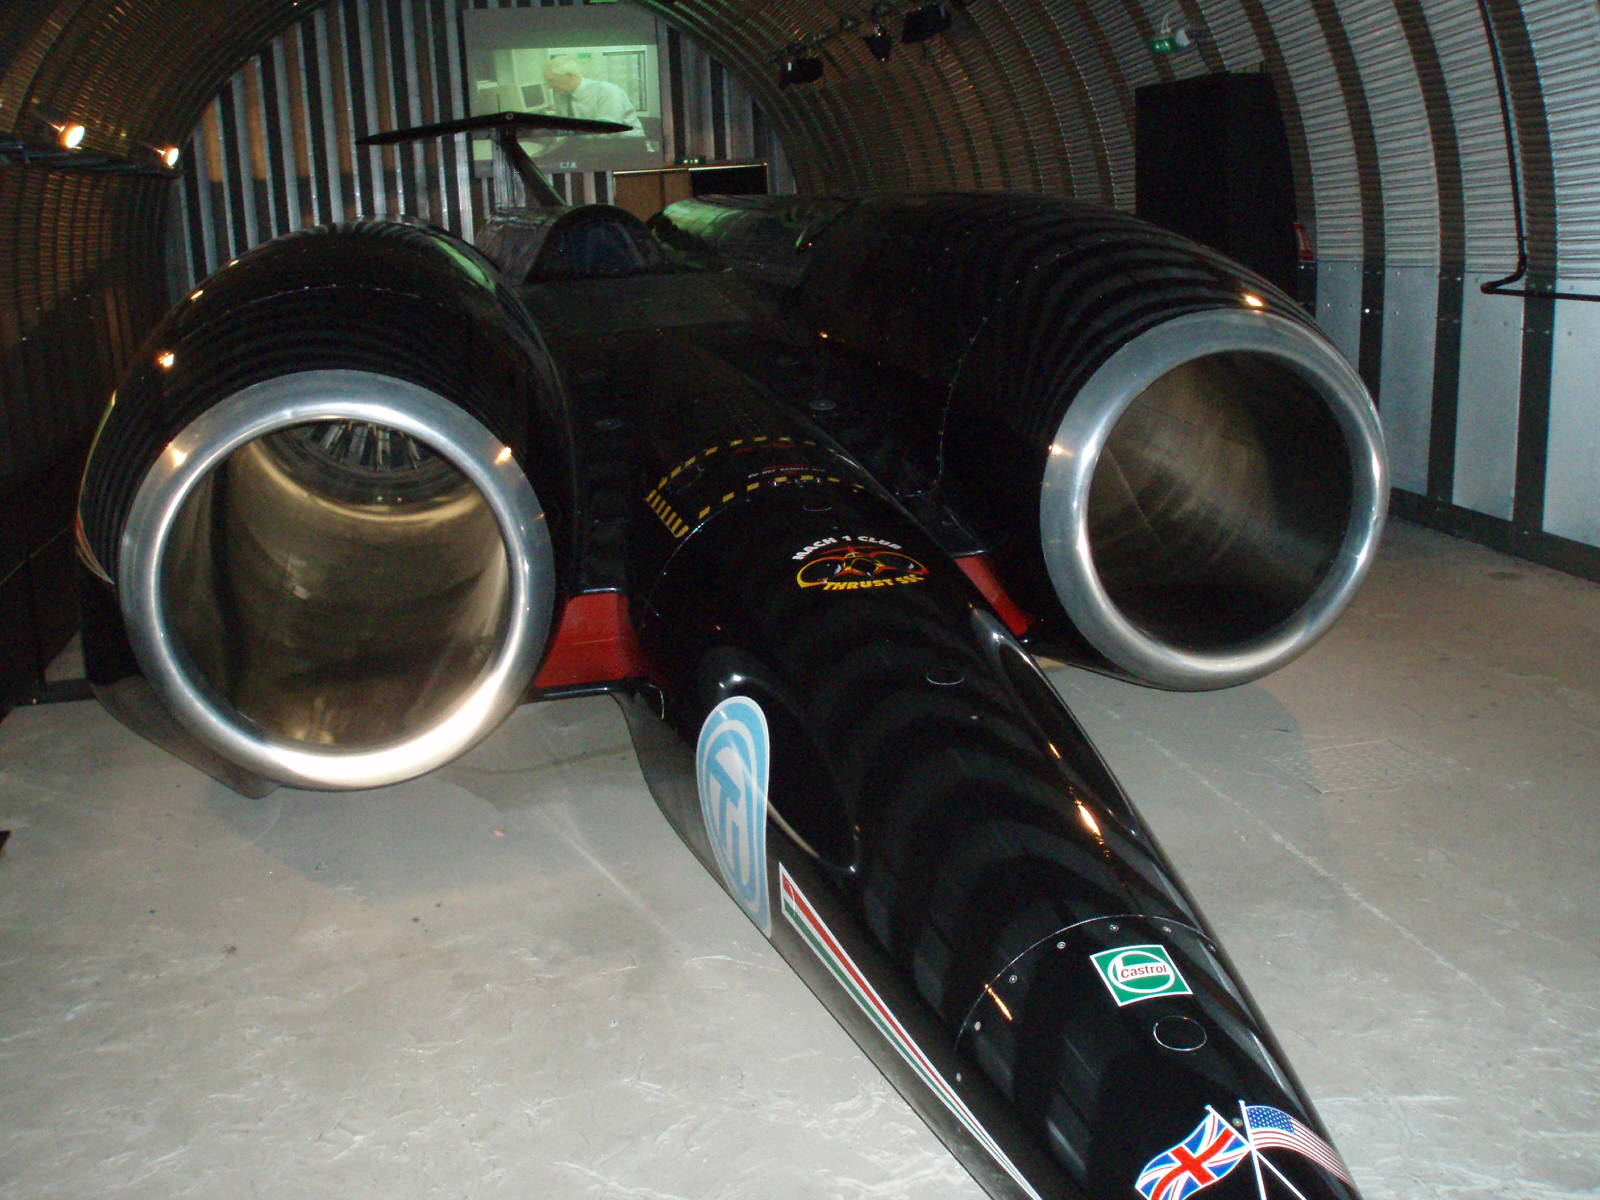
\includegraphics[height=4cm]{Clipart/ThrustSSC}
\index{ 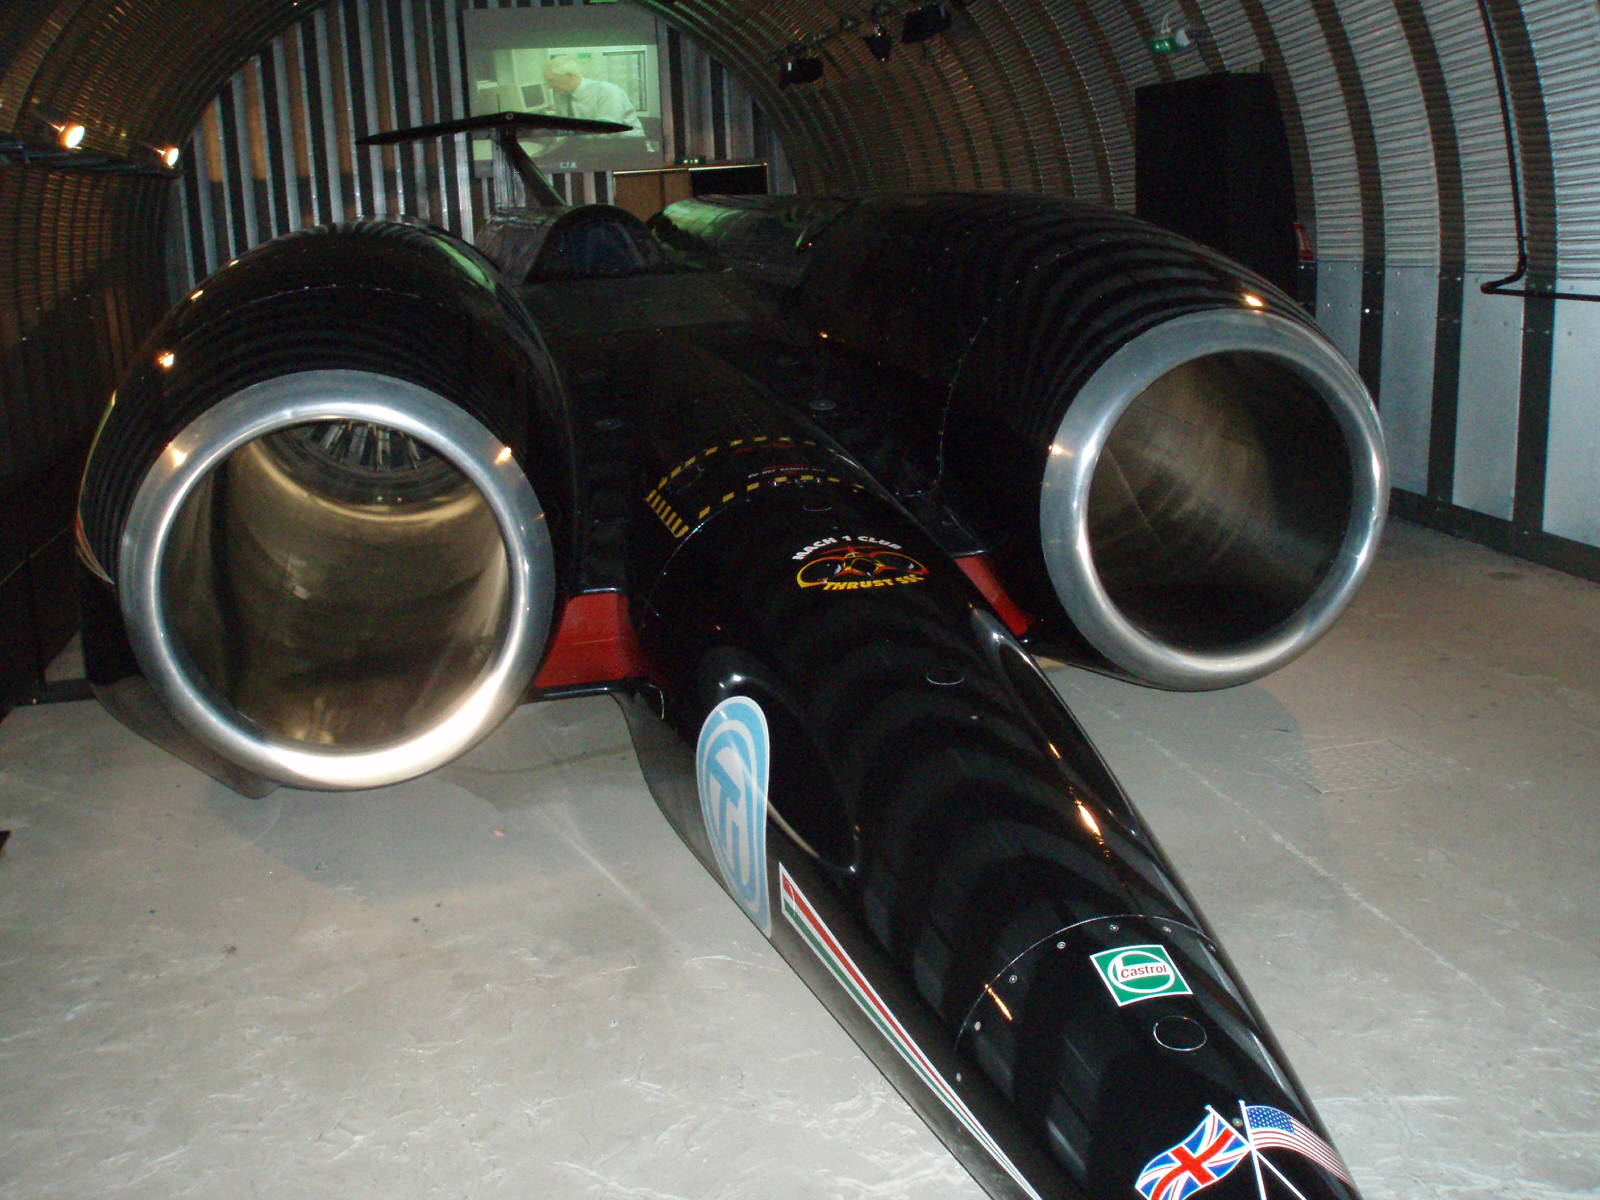
\includegraphics[height=5mm]{Clipart/ThrustSSC}
\href{https://en.wikipedia.org/wiki/Land_speed_record}{`ThrustSSC'}
by
\href{https://commons.wikimedia.org/wiki/User:Anonymous101}{Anonymous101}
is in the 
public domain (accessed 5 November 2015)}
\vfill
}
%
\SetQuestion{\AnswerYes
Suppose you want to download a file that is 3000 MB (slightly under 3GB). Your internet provider guarantees you that your download speeds will always be between 1 MBPS (MB per second) and  5 MBPS (because you bought the cheap plan). Using the Mean Value Theorem, give an upper and lower bound for how long the download can take (assuming your providers aren't lying, and your device is performing adequately).

}
\SetAnswer{\color{answercolor}
We assume the download is continuous and differentiable, so we can use the MVT. 

Let $T$ be the time (in seconds) the download takes. The MVT tells us that at some point, our speed was exactly $\frac{3000}{T}$, so it must be true that 
\[1 \leq \frac{3000}{T} \leq 5\] 
So, $\frac{3000}{5} \leq T \leq 3000$. That is, $T$ is between $600$ and $3000$ seconds, or between $10$ and $50$ minutes.
}
%
\SetQuestion{\AnswerYes
Suppose $1 \leq f'(t) \leq 5$ for all values of $t$, and $f(0)=0$. What are the possible solutions to $f(t)=3000$?\pause

Notice: since the derivative exists for all real numbers, $f(x)$ is differentiable and continuous for all real numbers!
}
\SetAnswer{\color{answercolor}
Since $f$ is continuous and differentiable, we can use the MVT. 

\[\frac{f(t)-f(0)}{t-0}=\frac{3000}{t}=f'(c)\]
for some value $c$ between $0$ and $t$.

So,
\[1 \leq \frac{3000}{t} \leq 5\]

hence
\[600 \leq t \leq 3000\]
}
\end{QuestionSet}
\end{frame}
%----------------------------------------------------------------------------------------
%----------------------------------------------------------------------------------------
%----------------------------------------------------------------------------------------

%----------------------------------------------------------------------------------------
\begin{frame}[t]
\note<1>{Explain what a ``corollary" is.}
\only<1>{\QuestionBar{1}{4}\AnswerYes}
\only<2>{\AnswerBar{1}{4}}
\begin{block}{Corollary to the MVT}
Let $a<b$ be numbers in the domain of $f(x)$ and $g(x)$, which are continuous over $[a,b]$ and differentiable over $(a,b)$.\\[1em]
\vfill\color{C1}
If $f'(x)=0$ for all $x$ in $(a,b)$, then \pause
\iftoggle{printsolutions}{\alert{$f(x)$ is constant in that interval. That is, $f(c)=f(d)$ for all $c,d$ in $[a,b]$.}}{\\[2em]~ }
\end{block}\vfill

\parbox{.3\textwidth}{
\begin{tikzpicture}
\draw (2,1) node(c)[vertex]{};
\draw (4,3) node(d)[vertex]{};

\color{M4}
\draw[C1,thick] (c) arc(180:90:2cm);
\draw (2.59,2.41) node[vertex](m){};
\draw[dashed] (c)--(d) (m)+(-.75,-.75) --+(.75,.75);
\end{tikzpicture}}
\color{answercolor}
\parbox{.6\textwidth}{
If $f(c) \neq f(d)$, then $\frac{f(d)-f(c)}{d-c} \neq 0$, so $f'(e) \neq 0$ for some $e$.
}\vfill

\unote{Corollary~\eref{text}{cor:DIFFmvtcons}}
\end{frame}
%----------------------------------------------------------------------------------------
\begin{frame}[t]
\only<1>{\QuestionBar{2}{4}\AnswerYes}
\only<2>{\AnswerBar{2}{4}}
\begin{block}{Corollary to the MVT}
Let $a<b$ be numbers in the domain of $f(x)$ and $g(x)$, which are continuous over $[a,b]$ and differentiable over $(a,b)$.\\[1em]
\vfill\color{C1}
 If $f'(x)=g'(x)$ for all $x$ in $(a,b)$, then \pause
\iftoggle{printsolutions}{\alert{$f(x)=g(x)+A$ for some constant value $A$.}}{\\[2em]~}
\end{block}
\vfill
\parbox{.3\textwidth}{
\begin{tikzpicture}
\foreach \y/\c in {0/C1,1/C4}{
\begin{scope}[yshift=\y cm]\color{\c}
\draw[ thick] plot[domain=-3.14:3.14]({\x/2},{sin(\x r)});
\draw[dashed,M4]  (-.5,-1) --(.5,1)node[midway,vertex]{};;
\end{scope}}
\end{tikzpicture}}
\color{answercolor}\hfill
\parbox{.6\textwidth}{
Define a new function $k(x) = f(x)-g(x)$. Then $k'(x)=0$ everywhere, so (by the last corollary) $k(x)=A$ for some constant $A$.}\vfill
\unote{Corollary~\eref{text}{cor equal diff}}
\end{frame}
%----------------------------------------------------------------------------------------
\begin{frame}[t]
\only<1>{\QuestionBar{3}{4}\AnswerYes}
\only<2>{\AnswerBar{3}{4}}
\begin{block}{Corollary to the MVT}
Let $a<b$ be numbers in the domain of $f(x)$ and $g(x)$, which are continuous over $[a,b]$ and differentiable over $(a,b)$.\\[1em]
\vfill\color{C1}
If $f'(x)>0$ for all $x$ in $(a,b)$, then \pause
\iftoggle{printsolutions}{\alert{$f(x)$ is increasing. That is, $f(c)<f(d)$ for all $c<d$ in $[a,b]$.}  }{\\[2em]~}
\end{block}\vfill

\parbox{.3\textwidth}{
\begin{tikzpicture}[yscale=-1]
\draw (2,1) node(c)[vertex]{};
\draw (4,3) node(d)[vertex]{};

\color{M4}
\draw[C1,thick] (c) arc(180:90:2cm);
\draw (2.59,2.41) node[vertex](m){};
\draw[dashed] (c)--(d) (m)+(-.75,-.75) --+(.75,.75);
\end{tikzpicture}}
\color{answercolor}
\parbox{.6\textwidth}{
If $f(c)>f(d)$ and $c<d$, then $\frac{f(d)-f(c)}{d-c}=\frac{\text{(negative)}}{\text{(positive)}}<0$. Then $f'(e)<0$ for some $e$ between $c$ and $d$.}
\vfill
\unote{Corollary~\eref{text}{cor:DIFFmvtcons}}
\end{frame}
%----------------------------------------------------------------------------------------
\begin{frame}[t]
\only<1>{\QuestionBar{4}{4}\AnswerYes}
\only<2>{\AnswerBar{4}{4}}
\begin{block}{Corollary to the MVT}
Let $a<b$ be numbers in the domain of $f(x)$ and $g(x)$, which are continuous over $[a,b]$ and differentiable over $(a,b)$.\\[1em]
\vfill\color{C1}
If $f'(x)<0$ for all $x$ in $(a,b)$, then \pause
\iftoggle{printsolutions}{\alert{$f(x)$ is decreasing. That is, $f(d)<f(c)$ for all $c<d$ in $[a,b]$.}  }{\\[2em]~}
\end{block}\vfill

\parbox{.3\textwidth}{
\begin{tikzpicture}[yscale=1]
\draw (2,1) node(c)[vertex]{};
\draw (4,3) node(d)[vertex]{};

\color{M4}
\draw[C1,thick] (c) arc(180:90:2cm);
\draw (2.59,2.41) node[vertex](m){};
\draw[dashed] (c)--(d) (m)+(-.75,-.75) --+(.75,.75);
\end{tikzpicture}}
\color{answercolor}
\parbox{.6\textwidth}{
If $f(c)<f(d)$ and $c<d$, then $\frac{f(d)-f(c)}{d-c}=\frac{\text{(positive)}}{\text{(positive)}}>0$. Then $f'(e)>0$ for some $e$ between $c$ and $d$.}
\vfill
\unote{Corollary~\eref{text}{cor:DIFFmvtcons}}
\end{frame}

%----------------------------------------------------------------------------------------

\begin{frame}[t]
\begin{block}{Mean Value Theorem -- Theorem~\eref{text}{thm:DIFFmvt}}

Let $f(x)$ be \textcolor{M3}{continuous} on the interval $[a,b]$ and \textcolor{M3}{differentiable} on $(a,b)$. Then there is a number $c$ strictly between $a$ and $b$ such that
\[ f'(c)=\textcolor{M4}{\frac{f(b)-f(a)}{b-a}}\]
\end{block}
\vfill

WARNING: The MVT has two hypotheses.
\begin{itemize}
\item $f(x)$ has to be continuous on $[a,b]$.
\item $f(x)$ has to be differentiable on $(a,b)$.
\end{itemize}
If either of these hypotheses are violated, the conclusion of the MVT can fail.
Here are two  examples.
\end{frame}

%----------------------------------------------------------------------------------------

\begin{frame}[t]
\begin{block}{Mean Value Theorem -- Theorem~\eref{text}{thm:DIFFmvt}}

Let $f(x)$ be \textcolor{M3}{continuous} on the interval $[a,b]$ and \textcolor{M3}{differentiable} on $(a,b)$. Then there is a number $c$ strictly between $a$ and $b$ such that
\[ f'(c)=\textcolor{M4}{\frac{f(b)-f(a)}{b-a}}\]
\end{block}
\vfill

Example: Let $a=-1$, $b=1$ and $f(x)=|x|$.

\begin{multicols}{2}
\begin{tikzpicture}[scale=0.75]
\myaxis{x}{3}{3}{y}{0}{3}
\draw[thick, C1] (-2,2)--(0,0);
\draw[thick, C1] (2,2)--(0,0);
\onslide<2-|handout:0>{\draw[dashed, M4] (-2,2)--(2,2);}
\draw (-2,2) node[vertex]{};
\draw (2,2) node[vertex]{};
\draw (2,.2)--(2,-.2) node[below]{$1$};
\draw (-2,.2)--(-2,-.2) node[below]{$-1$};
\end{tikzpicture}
\columnbreak\color{answercolor}
\onslide<3|handout:0>{
\begin{align*}
f'(x)=\begin{cases}
         1&\text{if }x>0\\
         -1&\text{if }x<0 \\
        \text{undefined}&\text{if }x=0
      \end{cases}
\end{align*}
$f'(x)$ is never $0=\frac{f(b)-f(a)}{b-a}$.}
\end{multicols}
\end{frame}
%----------------------------------------------------------------------------------------

\begin{frame}[t]
\begin{block}{Mean Value Theorem -- Theorem~\eref{text}{thm:DIFFmvt}}

Let $f(x)$ be \textcolor{M3}{continuous} on the interval $[a,b]$ and \textcolor{M3}{differentiable} on $(a,b)$. Then there is a number $c$ strictly between $a$ and $b$ such that
\[ f'(c)=\textcolor{M4}{\frac{f(b)-f(a)}{b-a}}\]
\end{block}
\vfill

Example: Let $a=0$, $b=1$ and 
$f(x)=\begin{cases}
        0&\text{if }x\le 0\\
        1&\text{if }x> 0
       \end{cases}$.

\begin{multicols}{2}
\begin{tikzpicture}[scale=0.75]
\myaxis{x}{1}{3}{y}{0}{3}
\draw[thick, C1] (2,2)--(0,2);
\draw[thick, C1] (-1,0)--(0,0);
\draw (0,0) node[vertex]{};
\draw (2,2) node[vertex]{};
\draw (2,.2)--(2,-.2) node[below]{$1$};
\onslide<2-|handout:0>{\draw[dashed, M4] (0,0)--(2,2);}
\end{tikzpicture}
\columnbreak\color{answercolor}
\onslide<3|handout:0>{
\begin{align*}
f'(x)=\begin{cases}
         0&\text{if }x>0\\
         0&\text{if }x<0 \\
        \text{undefined}&\text{if }x=0
      \end{cases}
\end{align*}
$f'(x)$ is never $1=\frac{f(b)-f(a)}{b-a}$.}
\end{multicols}
\end{frame}
%----------------------------------------------------------------------------------------
